\documentclass[journal]{IEEEtran}

%\documentclass[10pt]{beamer}
%\usepackage[left=1in,top=1in,right=1in,bottom=1in]{geometry}
\newcommand*{\authorfont}{\fontfamily{phv}\selectfont}
\usepackage{lmodern}

\usepackage{animate}
\usepackage[T1]{fontenc}
\usepackage{blindtext}
\usepackage{graphicx}
\usepackage{booktabs} % For formal tables
\usepackage{amsbsy}
\usepackage[ruled]{algorithm2e} % For algorithms
\usepackage{multirow}
\usepackage{amssymb}
\usepackage{amsmath}
\usepackage{tikz}
\usepackage[utf8]{inputenc}
\usepackage[english]{babel}
\usepackage{color}
\usepackage{soul}
\usepackage{fancyhdr}
\usepackage{float}
\usepackage{hyperref} 

\usepackage{amsthm}
\usepackage{mathtools}
\usepackage{xcolor}
\usepackage{pgfplots}
\usepackage{pdfpages}

\usepackage{verbatim}
\pgfplotsset{compat=1.17} 
\DeclarePairedDelimiter{\ceil}{\lceil}{\rceil}
\makeatletter
\def\thm@space@setup{%
  \thm@preskip=8pt plus 2pt minus 4pt
  \thm@postskip=\thm@preskip
}
\makeatother


%\newtheorem{theorem}{Theorem}[section]
%\newtheorem{corollary}{Corollary}[theorem]
%\newtheorem{lemma}[theorem]{Lemma}
%\newtheorem{definition}{Definition}[section]
\usetikzlibrary{automata, positioning}
\renewcommand{\algorithmcfname}{ALGORITHM}
\providecommand{\tightlist}{%
  \setlength{\itemsep}{0pt}\setlength{\parskip}{0pt}}

\fancypagestyle{firstpage}{% Page style for first page
  \fancyhf{}% Clear header/footer
  \renewcommand{\headrulewidth}{0.0pt}% Header rule
  \renewcommand{\footrulewidth}{0.0pt}% Footer rule
  \fancyhead[R]{\footnotesize{\thepage}}
  % Header
  %\fancyfoot[C]{-~\thepage~-}% Footer
}

%\ifCLASSINFOpdf
%\else
%\fi








%

\title{Simplified combinatorical analysis of burst failures \author{Serkay Ölmez \thanks{email: \href{mailto:serkay.olmez@seagate.com}{\nolinkurl{serkay.olmez@seagate.com}}}}  }

 



%\author{\Large \vspace{0.05in} \newline\normalsize\emph{}  }


\usepackage{setspace}


% set default figure placement to htbp


\usepackage{hyperref}
\usepackage{caption}
\usepackage{float}
\usepackage{graphicx}







% add some other packages ----------

% \usepackage{multicol}
% This should regulate where figures float
% See: https://tex.stackexchange.com/questions/2275/keeping-tables-figures-close-to-where-they-are-mentioned
\usepackage[section]{placeins}



\begin{document}
\onecolumn
% \pagenumbering{arabic}% resets `page` counter to 1 
%    

% \maketitle

{% \usefont{T1}{pnc}{m}{n}
\setlength{\parindent}{0pt}
\thispagestyle{plain}
{\fontsize{18}{20}\selectfont\raggedright 
\maketitle  % title \par  

}


}










\begin{abstract}


\noindent Calculating data loss probability under bursts of failures.

\vskip 8.5pt
%\begin{IEEEkeywords}
%combinatorics
%\end{IEEEkeywords}



\end{abstract}


\vskip -8.5pt


 % removetitleabstract

\noindent  

\hypertarget{TOC}{}

\hypertarget{the-set-up}{%
\section{The set up}\label{the-set-up}}

Consider \(N\) drives such that \(N=n_\text{i}\times n_\text{o}\), where the subscript \emph{o} is the short for \emph{outer} and \emph{i} is the short for \emph{inner}. Take \(n_\text{i}\) drives and apply an erasure coding with \(n_\text{i}=d_\text{i}+p_\text{i}\), where \(d_\text{i}\) stands for data drives and \(p_\text{i}\) stands for parity drives. This inner layer of erasure coding in this group of drives is capable of recovering from \(p_\text{i}\) simultaneous failures. Note that the number of such groups is \(n_\text{o}\). We can now that this already erasure coded groups and create another erasure coding on top with \(n_\text{o}=d_\text{o}+p_\text{o}\). With this set up, we would like to study the resiliency of the data against failure bursts, i.e., will the data survive if \(N_\text{f}\) drives fail all at the same time?

It will take at least \(p_\text{i}+1\) simultaneous failures for the inner layer to lose data. And we have to lose \(p_\text{o}+1\) inner layers for the outer layer to lose data. Therefore the minimum number of failures that can cause data loss is:
\begin{eqnarray}
n_\text{min}=(p_\text{i}+1)\times (p_\text{o}+1)
\label{eq:nmindef}
\end{eqnarray}

\hypertarget{counting-combinations}{%
\section{Counting combinations}\label{counting-combinations}}

Consider the first of the erasure coded inner layer group that consists of \(n_\text{i}\) drives, and assume there are \(f_0\) failed drives in this group where \(0\leq f_0\leq n_\text{i}\). The total number of creating a configuration with \(f_0\) failed and \(n_\text{i}-f_0\) healthy drives is:
\begin{eqnarray}
\mathcal{C}(f_0)=\frac{n_\text{i}!}{(n_\text{i}-f_0)!f_0!} .
\label{eq:pb0}
\end{eqnarray}
We need to repeat this for all inner groups and multiply them together to get the total number of combinations

\begin{eqnarray}
\mathcal{C}(f_0,f_1,\cdots, f_{n_\text{o}-1})&=& {\displaystyle \prod_{k=0}^{n_\text{o}-1}} \mathcal{C}(f_k)={\displaystyle \prod_{k=0}^{n_\text{o}-1}} \frac{n_\text{i}!}{(n_\text{i}-f_k)!f_k!}
=\left(n_\text{i}!\right)^{n_\text{o}}{\displaystyle \prod_{k=0}^{n_\text{o}-1}} \frac{1}{(n_\text{i}-f_k)!f_k!}.
\label{eq:tcf}
\end{eqnarray}
Equation \eqref{eq:tcf} is the total number of combinations for an arbitrary collection of failures per inner layer, i.e., \(\{f_0,f_1,\cdots, f_{n_\text{o}-1}\}\) with the only constraint being \(0\leq f_k\leq n_\text{i}\). We want to consider cases where the total number of failed drives is a fixed number by imposing the following condition on \(f_k\):
\begin{eqnarray}
 \sum_{k=0}^{n_\text{o}-1}f_k= N_\text{f}.
\label{eq:fsum}
\end{eqnarray}
We can now sum over every possible value of \(f_k\) satisfying Eq. \eqref{eq:fsum} to get the total number of combinations with total \(N_\text{f}\) failed drives.
\begin{eqnarray}
\mathcal{C}&=& \sum_{f_0}\sum_{f_1}\cdots \sum_{f_{n_\text{o}-1}} \mathcal{C}(f_0,f_1,\cdots, f_{n_\text{o}-1}) \delta\left(  \sum_{l=0}^{n_\text{o}-1}f_l- N_\text{f}\right)\nonumber\\
&=& \left(n_\text{i}!\right)^{n_\text{o}}  \sum_{f_0}\sum_{f_1}\cdots \sum_{f_{n_\text{o}-1}} {\displaystyle \prod_{k=0}^{n_\text{o}-1}} \frac{1}{(n_\text{i}-f_k)!f_k!} \delta\left(  \sum_{l=0}^{n_\text{o}-1}f_l- N_\text{f}\right),
\label{eq:tcfs}
\end{eqnarray}
where we imposed the condition in Eq. \eqref{eq:fsum} using the Kronecker delta function, \(\delta\).

For computational purposes, we can eliminate the eliminate Kronecker delta function by carefully defining the range of the summation indices, i.e., \(f_k\) so that Eq. \eqref{eq:fsum} is satisfied by definition:
\begin{eqnarray}
\mathcal{C}&=& \left(n_\text{i}!\right)^{n_\text{o}}  \sum_{f_0=0}^{N_\text{f}}\sum_{f_1=0}^{N_\text{f}-f_0}\cdots \sum_{f_{n_\text{o}-2}=0}^{N_\text{f}-\sum_{l=0}^{n_\text{o}-3}f_l} {\displaystyle \prod_{k=0}^{n_\text{o}-1}} \frac{1}{(n_\text{i}-f_k)!f_k!}\bigg\rvert_{f_{ n_\text{o}-1=N_\text{f}-\sum_{l=0}^{n_\text{o}-2}f_l}}.
\label{eq:tcfs2}
\end{eqnarray}
Note that we can use this equation as is although the summation indices \(f_k\) may exceed \(n_\text{i}\). For those cases we will get \(0\) from the product term since negative factorials ,\(f_k>n_\text{i}\), become infinite. For numeric computations, the upper range of the summation \(f_k\) can be truncated at \(\min(N_\text{f}-\sum_{l=0}^{k-1}f_l, n_\text{i})\).

\hypertarget{counting-data-loss-instances}{%
\section{Counting data loss instances}\label{counting-data-loss-instances}}

Not all of these combinations result in data loss. If \(f_k>p_\text{i}\) then the inner layer \(k\) has lost data. And if the number of inner layers that lost data is larger than \(p_\text{o}\), the overall system has lost data. We can put this in using nested \(\Theta\) functions:

\begin{eqnarray}
\text{Data Loss}&=& \Theta\left[  \sum_{l=0}^{n_\text{o}-1}  \Theta \left[f_l-p_\text{i} \right]-p_\text{o}     \right],
\label{eq:theta}
\end{eqnarray}
where \(\Theta[m]\) returns \(1\) for \(m\geq 1\) and \(0\) otherwise.

\hypertarget{probability-of-data-loss}{%
\section{Probability of data loss}\label{probability-of-data-loss}}

We have been counting the combinations that give data loss cases. We need to normalize that against total number of combinations with \(N_\text{f}\) failed and \(N-N_\text{f}\) healthy drives which is simply:

\begin{eqnarray}
\mathcal{C}_\text{T}=\frac{N!}{(N-N_\text{f})!N_\text{f}!}.
\label{eq:pb0}
\end{eqnarray}

And finally, the probability of losing data becomes:

\begin{eqnarray}
\mathcal{P}&=&\frac{\mathcal{C}_\text{DL}}{\mathcal{C}_\text{T}}\nonumber\\
&=& \frac{(N-N_\text{f})!N_\text{f}! \left(n_\text{i}!\right)^{n_\text{o}}}{ N!}  \sum_{f_0=0}^{N_\text{f}}\sum_{f_1=0}^{N_\text{f}-f_0}\cdots \sum_{f_{n_\text{o}-2}=0}^{N_\text{f}-\sum_{l=0}^{n_\text{o}-3}f_l} {\displaystyle \prod_{k=0}^{n_\text{o}-1}} \frac{\Theta\left[  \sum_{l=0}^{n_\text{o}-1}  \Theta \left[f_l-p_\text{i} \right]-p_\text{o}     \right]}{(n_\text{i}-f_k)!f_k!}\bigg\rvert_{f_{ n_\text{o}-1=N_\text{f}-\sum_{l=0}^{n_\text{o}-2}f_l}}.
\label{eq:ploss}
\end{eqnarray}

Numerically evaluating Eq. \eqref{eq:ploss} is somewhat convoluted due to the changing number of summations as \(n_\text{o}\) changes. Below are the result for probability of losing data vs number of failures for selected erasure coding as shown in the title. Two traces (which are on top of each other) show the results from brute force counting and the formula. The code is somewhat hard coded to handle \(n_\text{o}=3\) case.

\begin{figure}[H]

{\centering 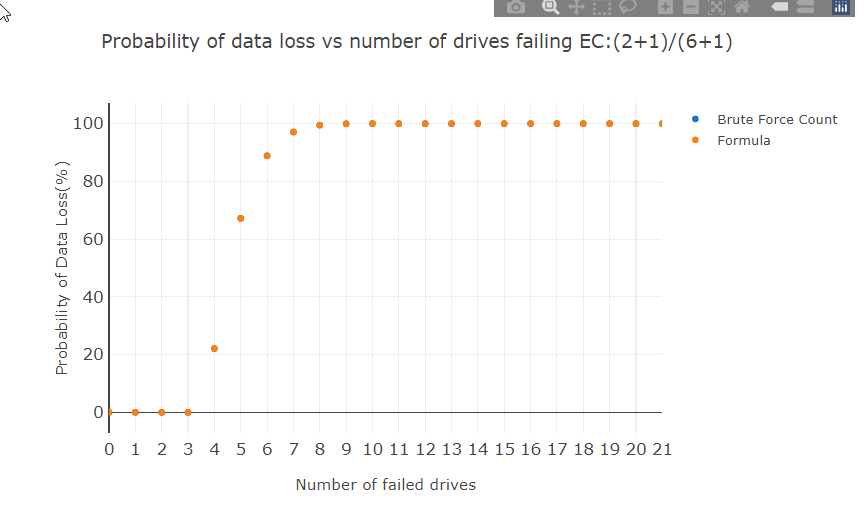
\includegraphics[width=0.65\linewidth]{2161} 

}

\caption{EC:(2+1)/(6+1)}\label{fig:2161}
\end{figure}

\begin{figure}[H]

{\centering 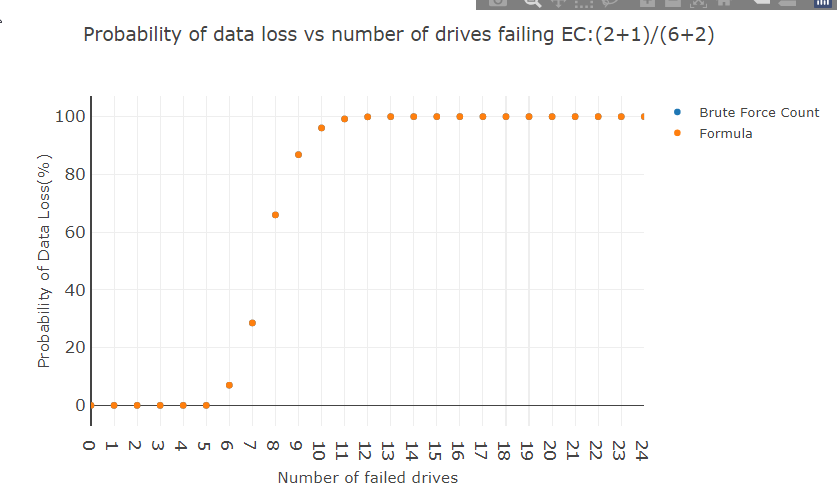
\includegraphics[width=0.65\linewidth]{2162} 

}

\caption{EC:(2+1)/(6+2)}\label{fig:2162}
\end{figure}

\begin{figure}[H]

{\centering 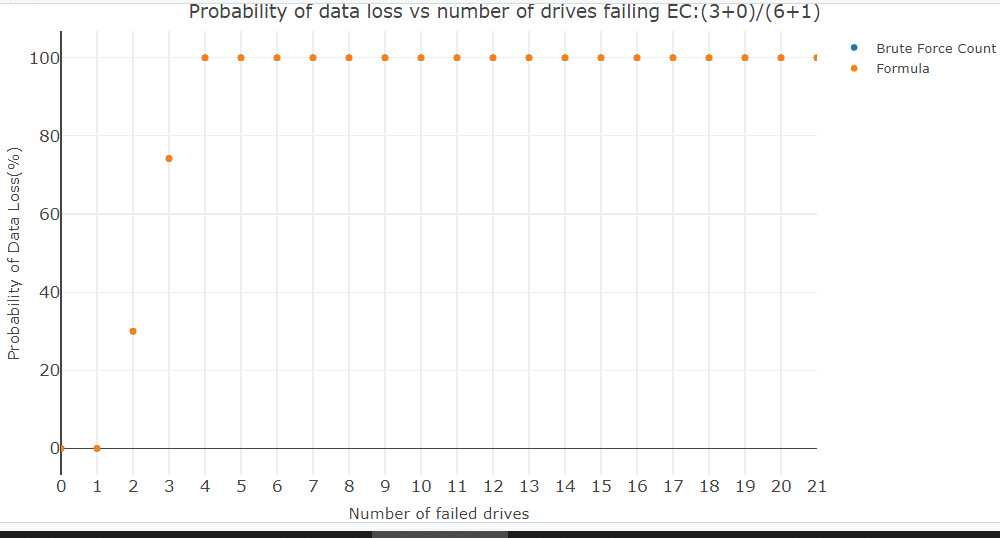
\includegraphics[width=0.65\linewidth]{3061} 

}

\caption{EC:(3+0)/(6+1)}\label{fig:3061}
\end{figure}

\begin{figure}[H]

{\centering 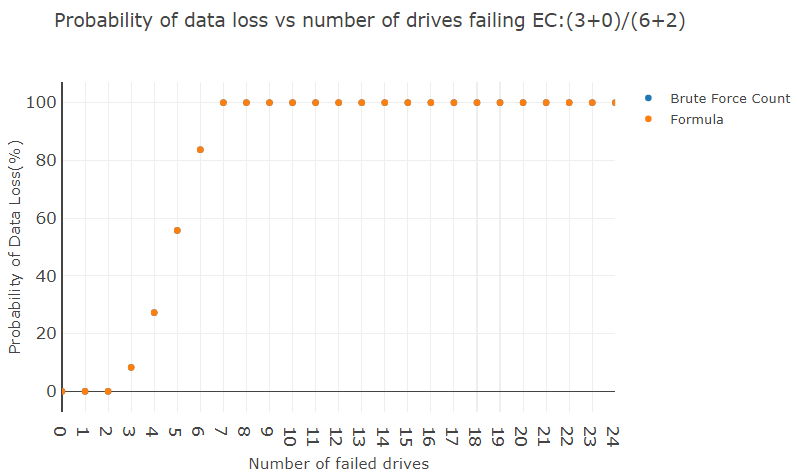
\includegraphics[width=0.65\linewidth]{3062} 

}

\caption{EC:(3+0)/(6+2)}\label{fig:3062}
\end{figure}

\newpage
\singlespacing 



\end{document}
